\section{Arequipa, Colca, Titicaca}

Date: 28/10/2009

\begin{multicols}{2}

Hola amigos !!

Voici le suite de mon voyage, aujourd'hui je vous emmène à Arequipa, dans le Sud du Pérou, puis au fond du Colca Cañon, le plus haut cañon du monde. Ensuite nous descendrons encore plus au sud en direction du lac Titicaca. Nous ferons une très courte halte a Puno, puis nous traverserons la frontière en direction de Copacabana en Bolivie. La Paz, d'où je vous écrit, sera le début du prochain article car j'attend d'être parti d'un endroit pour en parler, pour être plus complet.

Destination donc Arequipa, deuxième plus grande ville du Perou avec son million d'habitants. Cette ville se détache du reste du Perou par sa propreté quasiment déconcertante lorsque l'on vient de la côte, plutôt arride, désertique et poussiéreuse. Arequipa est nichée au pied de plusieurs volcans, dont le Misti qui culmine a plus de 6000 mètres d'altitude.

Voici une photo pour vous donner une petite idee de ce volcan magnifique, nous nous sommes demandés si on faisait un trek de deux jours pour monter au sommet avec Didier puis je me suis très rapidemnent dégonflé, lui un peu après, cela aurait quand meme fait 3500 mètres de dénivelé à grimper en deux jour avec tout ce que cela implique, dont le manque d'air.

\hspace*{-0.65cm}
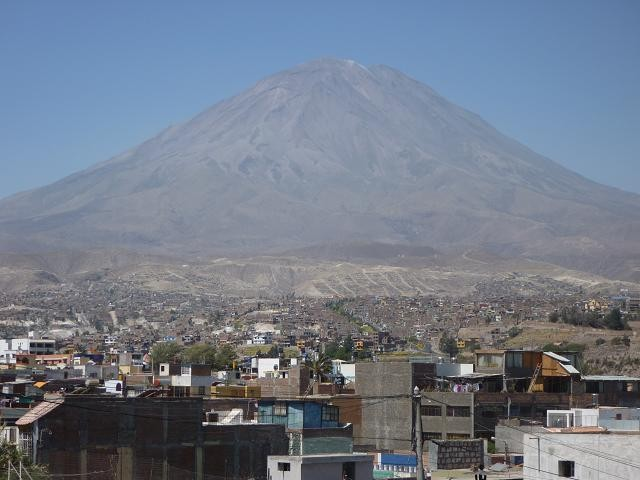
\includegraphics[width=4.8cm]{articles/Arequipa-colca-titicaca/1256606928TSDk.jpg}
Le Misti tout près d'Arequipa

Je me rend compte que pour l'instant vous n'avez pas vraiment encore vu comment sont les péruviens, je vais donc essayer de vous mettre quelques photos dans cet article pour que vous vous en rendiez mieux compte. Même si le côté humain du voyage ne peut pas se raconter, et c'est pour ca que je n'essai que très peu de le faire, je pense important d'essayer de vous montrer l'ambiance dans laquelle je suis plongé au jour le jour.

Nous commençons par un bonhomme, bien sympa, a l'entrée d'un petit église en haut d'Arequipa. J'ai passe une petite demi heure avec lui à discuter, il m'a même parlé de Robespierre.. et n'oublie pas de tendre la main pour avoir une petite pièce. Je vous presente donc José.

\hspace*{-0.65cm}
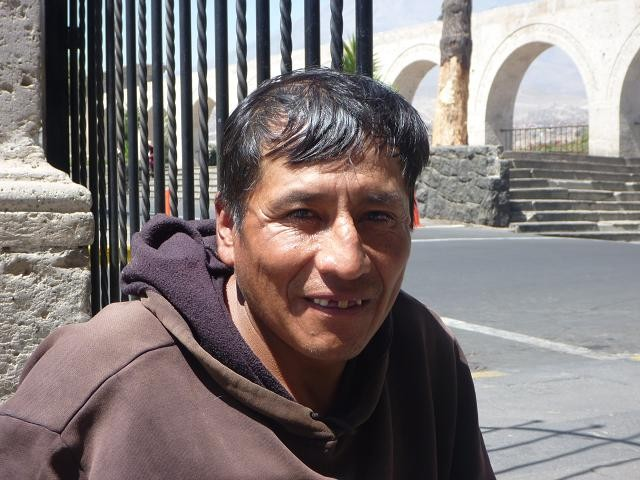
\includegraphics[width=4.8cm]{articles/Arequipa-colca-titicaca/1256606933jPp4.jpg}
José, le mec qui en sait plus sur l'histoire de France que beaucoup de nous

Après être restés deux jours à Arequipa, nous décidons avec Didier d'aller voir le cañon de Colca, le plus profond du monde. Nous prenons un bus à une heure du matin en pensant pouvoir dormir dedans et ainsi économiser une nuit d'hôtel. C'était sans compter sur la route (enfin, route, tout est relatif..) qui mène à Cabanaconde. Imaginez un bus aux vitre brenlantes roulant avec grand bruit sur une piste tres cahoteuse, resultat : une nuit blanche. Nous arrivons a Cabanaconde, à mi hauteur du cañon à peux près, nous zonons un petit peu puis posons notre sac dans une chambre d'hôtel. La vue des lits nous incite à dormir deux heure, puis on attaque la descente.. c'est parti pour 1h50 de descente pour franchir les 1100 mètres de dénivelé qui nous séparent de la piscine se trouvant dans l'oasis, en bas.

\hspace*{-0.65cm}
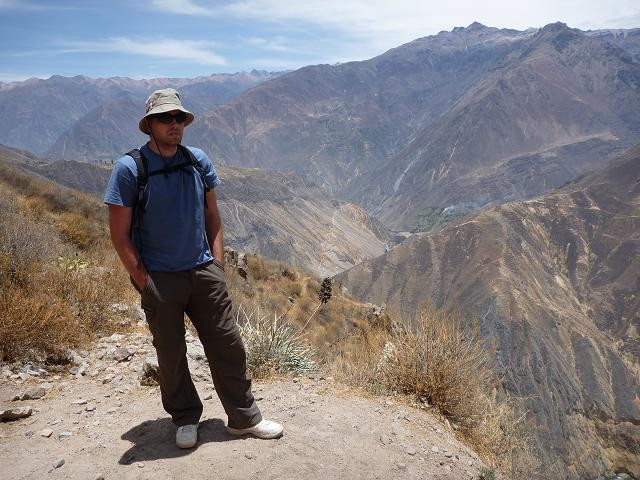
\includegraphics[width=4.8cm]{articles/Arequipa-colca-titicaca/12566073542gHb.jpg}
A un mètre, c'est chute libre jusqu'en bas...

Destination l'oasis..

\hspace*{-0.65cm}
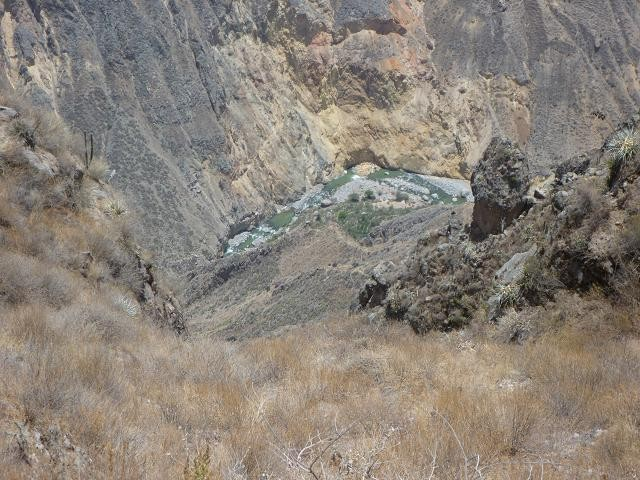
\includegraphics[width=4.8cm]{articles/Arequipa-colca-titicaca/1256607360xfpT.jpg}
... ouais ici, là, en bas

Encore une super vue.

\hspace*{-0.65cm}
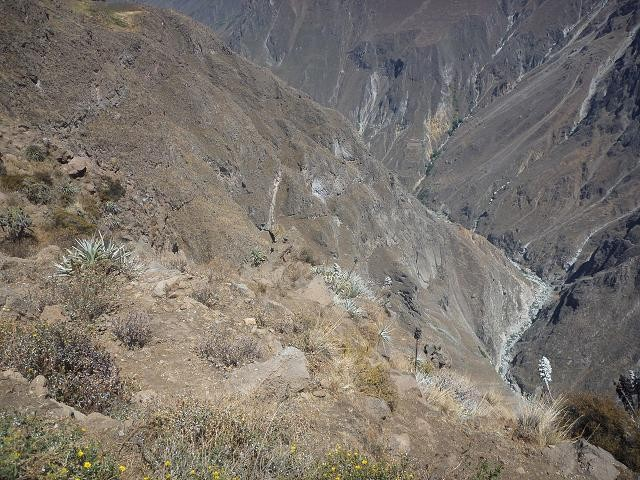
\includegraphics[width=4.8cm]{articles/Arequipa-colca-titicaca/1256607348QGMH.jpg}
Sympa ce cañon

Apres un petit plouf d'une bonne heure dans la piscine du bas, nous voici partis pour remonter, le plus dur !! Nous avons mis 3 heures pour franchir les 1100 mètres de déniveléé en sens inverse. Si j'insiste sur la hauteur c'est parce que c'est réélement impressionnant de voir ça, monter quasi à la vertical sur plus d'un kilomètre. C'est bien simple, une fois arrivé j'avais plus de genous. Une journée bien remplie.

Un truc hallucinant que nous avons vu, les locaux utilisent des ânes pour monter, vue l'étroitesse du chemin, les éboulis constants et le fait que les ânes n'aient pas la notion du risque et donc tournent au dernier moment, je trouve ca complètemnent suicidaire.

\hspace*{-0.65cm}
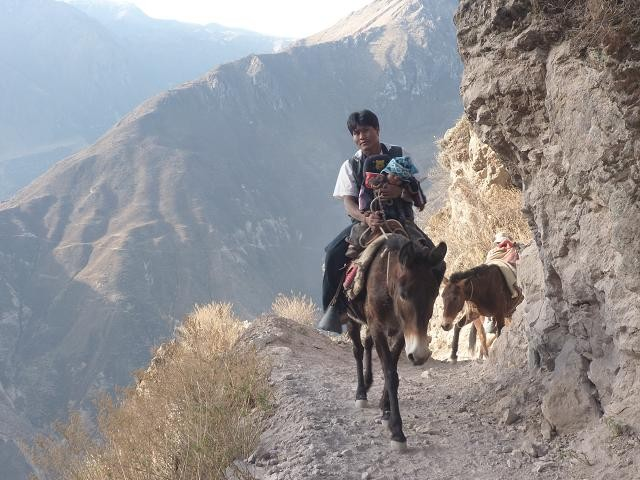
\includegraphics[width=4.8cm]{articles/Arequipa-colca-titicaca/1256607366kAzy.jpg}
No stress, normal

Rien que pour vous, une petite photo qui a du piquant.

\hspace*{-0.65cm}
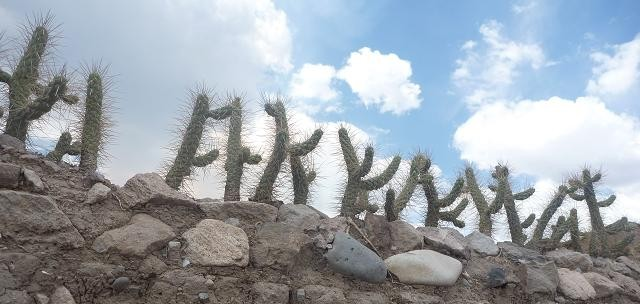
\includegraphics[width=4.8cm]{articles/Arequipa-colca-titicaca/1256607370Azvi.jpg}
Des plantes vertes avec des cure dents plantés dedans. Quoi ? Comment dites vous ? Cactus ? Ah bon !

Au revoir Arequipa, vamos a Puno, ville péruvienne sur les bords du lac Titicaca. Le principal intérêt touristique de Puno est d'aller voir des îles flottantes faites en bambous sur lesquelles vivent des gens. En fait ça ne m'attirait pas trop, et ce que j'en ai entendu dire est que le tourisme a pervertie cet endroit, le folklore devient supercherie. J'ai donc préféré me ballader dans les rues, et donc évidement au marché.

\hspace*{-0.65cm}
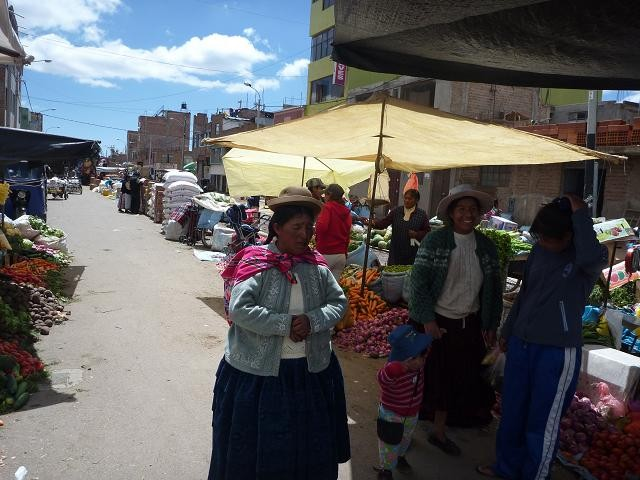
\includegraphics[width=4.8cm]{articles/Arequipa-colca-titicaca/12566069210hdx.jpg}
Marché de Puno

Nous passons maintenant la frontière Bolivienne pour aller à Copacabana situé sur une presqu'ile au Sud-Est du lac Titicaca. Petit ville très sympa, calme, mais une fois encore un peu trop touristique à mon goût au centre ville. Les habitants de Copacabana ont une perticularité très.. particulière. Ils font bénir des petites voitures et maisons (taille jouet) dans l'espoir d'avoir le model grandeur nature dans l'année. Alors vient la bénédiction des voitures (vraies cette fois). Assister à cela est étrange.

\hspace*{-0.65cm}
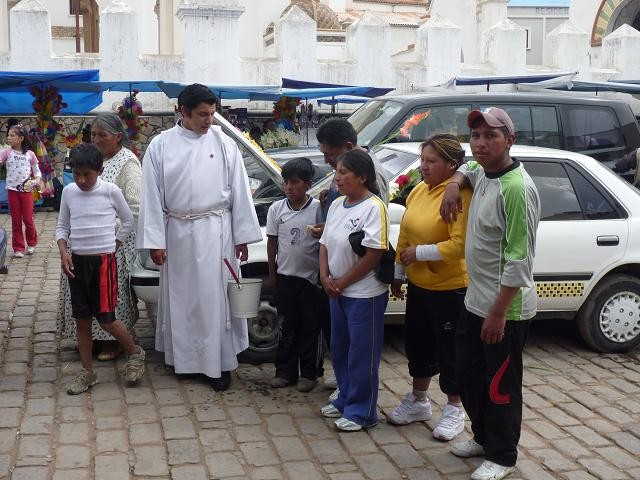
\includegraphics[width=4.8cm]{articles/Arequipa-colca-titicaca/1256606967Syll.jpg}
Le prêtre de Copacabana qui béni les voitures de ses ouailles

Voici une vue du lac Titicaca du haut d'une colline bordant Copacabana. La grimpette pour monter, pourtant pas très haute (100m de dénivelé) est très fatiguante, car a 3900m d'altitude, qui correspond à l'altitude du lac, le manque d'air essoufle très vite.

\hspace*{-0.65cm}
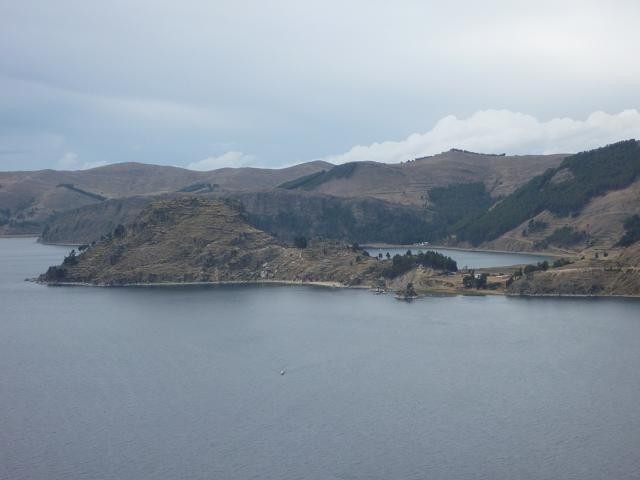
\includegraphics[width=4.8cm]{articles/Arequipa-colca-titicaca/125660697038LL.jpg}
Le lac Titicaca

Une petite photo inter générationnelle, prise dans les rues de la ville.

\hspace*{-0.65cm}
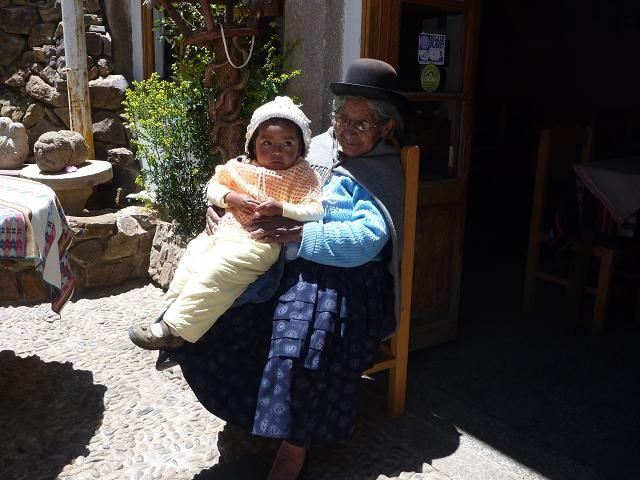
\includegraphics[width=4.8cm]{articles/Arequipa-colca-titicaca/1256606974OTlv.jpg}
Une super photo que j'ai failli pas pouvoir prendre à cause de mon espagnole approximatif

Allez, c'est décidé, je m'écarte un peu du centre ville, je vais voir autour. Je tombe sur une compétition de foot réunissant des équipes boliviennes et péruviennes, assurant le spectacle sur toute la journée, du moins avant la pluie. En fait d'assister à tous les matchs, je vais à l'exterieur de l'enceinte où je rencontre un groupe d'hommes, occupés à vider des bières. Ils m'invitent à pratiquer ce sport moins populaire que le foot mais tout aussi sympatique en temps de grandes chaleures, on pratique donc le lever de coude un bon moment, en discutant, puis je sors mes balles de jonglages et c'est reparti de plus belles.

\hspace*{-0.65cm}
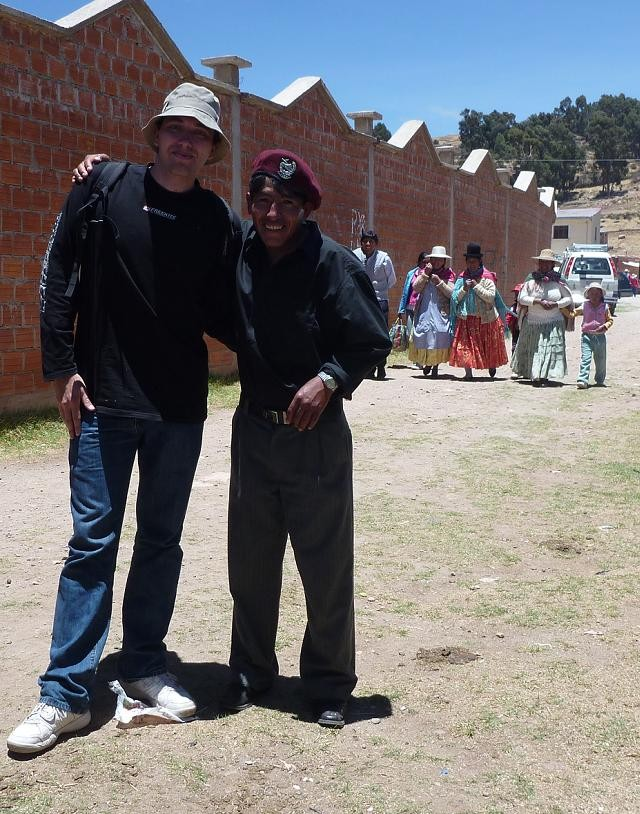
\includegraphics[width=4.8cm]{articles/Arequipa-colca-titicaca/1256606985kcoP.jpg}
Ici en revanche pas de problème d'éspagnol, en fait on a surtout travaillé la gnole, mais pas trop l'Espagne

Plus tard, je passe devant un batiment d'ou sortent des bruits d'echo me rappelant le bowling, il faut que je vois ça, je rentre et il s'agit en fait de squash. C'est parti pour taper dans la balle avec le mec qui gère la salle. Je ne vous dirais pas qui a gagné mais simplement que sur deux parties de 40 points j'en ai mis 80, alors que lui est censé être habitué à l'altitude. Il est tout aussi crevé que moi à la fin. 1 heure de squash à 4.000 mètres d'altitude, si vous voulez cracher vos poumons, je conseil !

Au moment où la France est passée à l'heure d'hiver, ici il fait toujours aussi chaud, nous approchons de l'été. Je vous laisse avec une petite photo intitulee "Cerveza sobre Titicaca".

\hspace*{-0.65cm}
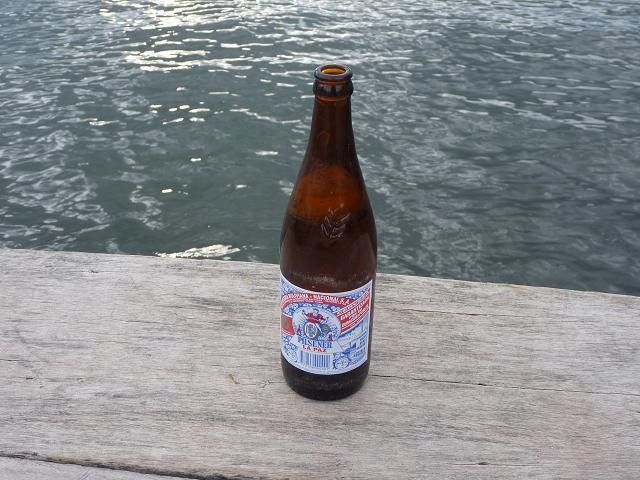
\includegraphics[width=4.8cm]{articles/Arequipa-colca-titicaca/1256606978ASqj.jpg}
Une petite bière au bord du lac Titicaca

Hasta luego..

\end{multicols}

\bigskip
\textbf{\textsc{Commentaires}}

\medskip
Titou et Chachou a écrit le 28 oct. 2009 :
\begin{displayquote}
Et bah voilà, il était pas trop tôt ! Content de voir que tu t'amuses et surtout que tu vas bien ! Bah oui hein on s'inquiétait un peu nous de l'autre côté de la planète :-)
Merci pour les jolies photos et pour les petits commentaires même si on en veut toujours plus !
Continue de t'amuser et de profiter de tes vacances, en faisant toujours bien gaffe à tes fesses.
Gros bisous de nous deux et à très bientôt !
\end{displayquote}

\medskip
Tatid a écrit le 30 oct. 2009 :
\begin{displayquote}
Waouh ça en jette\dots pendant que d'autres bossent, et de temps en temps, jusqu'à 1h30 du mat' ! Quand on voit ton blog, on se dit "punaise, qu'est-ce que je fous ici" ! :-)
Profite bien ami Dud et reviens tout bronzééé !
\end{displayquote}

\medskip
Tatid a écrit le 30 oct. 2009 :
\begin{displayquote}
J'en profite d'être sur ce blog pour te dire Fab qu'il faut qu'on se fasse un truc un de ces 4, ça fait trop longtemps qu'on s'est pas vu :-)
\end{displayquote}

\medskip
Etienne a écrit le 31 oct. 2009 :
\begin{displayquote}
Hey hey, pour avoir une autre version de cet article, en plus long et avec un autre style, allez voir le blog de Didier, <a href="http://didieroncareerbreak.typepad.com/didiers-career-break/2009/10/arequipa-canyon-de-colca.html">c'est par là</a>, et c'est bien sympa.
\end{displayquote}

\medskip
Titou et Chachou a écrit le 31 oct. 2009 :
\begin{displayquote}
Hey Hey ! Merci pour ces news sur le blog et par mail ! Avec le blog de Didier on aura de la lecture en plus pour nos longues soirées et journées :p

Continue de t'amuser et à très bientôt !
Bisous de nous deux !
A plutch
\end{displayquote}

\medskip
Sonia a écrit le 31 oct. 2009 :
\begin{displayquote}
Coucou etienne
Alors je te découvre aventurier, écrivain, voyageur\dots Que de belles révélations!
L'histoire du chandelier me laisse perplexe /:~)
bref profite un max et a bientôt
\end{displayquote}

\medskip
Grand-mère a écrit le 1 nov. 2009 :
\begin{displayquote}
Bonsoir Etienne,
Nous avons lu ton journal de bord avec beaucoup d'intérêt, et admiré tes photos! Magnifique! profites-bien de ton voyage, de tes rencontres! Nous te suivons par la pensée!
Grand-mère, Monique et Alain
\end{displayquote}

\medskip
Jaco a écrit le 1 nov. 2009 :
\begin{displayquote}
Bien content de voir que tout continue à bien se passer !
Reviens nous vite quand même qu'on lève le coude ensemble ;)
Bisous vieux fou
\end{displayquote}

\medskip
Didier a écrit le 4 nov. 2009 :
\begin{displayquote}
Tu vois que tout se résume à boire un bon coup pour faire plus ample connaissance avec la faune locale :-)
J'aime bien aussi le coup du squash, je te prends quand tu veux\dots
Sinon de mon côté je viens de terminer le chemin des Incas, du tout bon! Même si c'était assez chaud au début (j'avais pris beaucoup trop de brol avec moi, du coup mon sac pesait 1 tonne).
Je pars du 5 au 8 nov dans la jungle et suis de retour à Cuzco le 9 avant de partir vers le lac Titicaca/La Paz and Co donc tiens moi au courant et avec un peu de chance on se boira une Cusqueña ici!
PS: je loge a l'hostal "The Point"
\end{displayquote}

\vfill

